\documentclass{bioinfo}
\copyrightyear{2005}
\pubyear{2005}

\begin{document}
\firstpage{1}

\title[short Title]{This is a title}
\author[Sample \textit{et~al}]{Corresponding Author\,$^{1,*}$, Co-Author\,$^{2}$ and Co-Author\,$^2$\footnote{to whom correspondence should be addressed}}
\address{$^{1}$Department of XXXXXXX, Address XXXX etc.\\
$^{2}$Department of XXXXXXXX, Address XXXX etc.}

\history{Received on XXXXX; revised on XXXXX; accepted on XXXXX}

\editor{Associate Editor: XXXXXXX}

\maketitle


\begin{abstract}

\section{Summary:}
 Numerous methods have been proposed to find the optimal partition of a signal in a given number of segments, but very few address the question of the quality of the segmentation. In many biological data-sets (CGH-array, NGS, ...),  each segment is assumed to be related to a biological event so that the certainty of their location and the number of segments is crucial. EBS is an R package that provides through a Bayesian framework exact quantities such as the posterior distribution of a change-point position, and an efficient ICL criterion for the selection of the total number of change-points. All quantities are computed in a quadratic time.


\section{Availability:}
EBS is available as an R package from CRAN repositories (e.g. http://cran.r-project.org/web/packages).


\section{Contact:} alice.cleynen@agroparistech.fr
\end{abstract}

\section{Introduction}

Change-point detection strategies include exact methods such as the Dynamic Programming Algorithm \citep{bellman_approximation_1961}, or fast and efficient heuristic such as Binary Segmentation \citep{breiman_cart}, but most do not address crucial questions like the quality of the segmentation or the uncertainty on the localisation of breakpoints. Those quantities could however be usefull when choosing the number of segments, or comparing the segmentation of different profiles. 

Recently, \cite{Luong_HMM_2012} proposed a method to estimate the posterior distribution of a breakpoint using a constrained HMM model. However, it relies on the input of segment parameters, thus does not explore the entire segmentation space. EBS is an implementation of the framework described in \cite{rigaill_exact_2011} which derives exact posterior probabilities of quantities such as the number of segments, the entropy of a segmentation, or the localisation of the change-points.



\section{Approach}

Our approach is valid for all models satisfying the factoriability assumption: if $Y$ denotes the data, $m$ a segmentation and $r$ a segment of $m$, 
\begin{equation}
 (H)\quad P(Y,m) = C \prod_{r\in m} a_r P(Y^r|r) \label{factoriability}
\end{equation}
where $P(Y^r|r) =\int P(Y^r|\theta_r)P(\theta_r)d\theta_r $. The package includes the Poisson, Normal Heteroscedastic and Negative Binomial (with known overdispersion parameter) models that all verify $(H)$.

The computation of the quantities of interest all rely on $P(Y,K)$ (K being the number of segments) that can be computed in quadratic time as
\begin{equation}
 P(Y,K) = \left[{n-1} \choose{K-1} \right]^{-1} \left(A^K \right)_{1,n+1} \label{Proba}
\end{equation} 
where $A_{i,j}=P(Y^{[\![i,j[\![})$. (See Proposition 2.2 of \cite{rigaill_exact_2011} for proof).

\begin{methods}

\section{Available Functionality}

Table \ref{Tab:01} gives the list of the functions available in the EBS Package. This section describes and illustrates their use with a continued example. 

\subsection{Initialization}

All quantities of interest can be computed using simple operations on the elements of the matrix $A$ of segment probabilities. The function \texttt{EBSegmentation} initializes this matrix with the data according to the user's choice of maximum number of segments and data-model. Each of them is associated with a prior distribution on the parameters (for instance, Gamma for the Poisson model), and the result depends on the value of the hyperparameters. By default \texttt{EBSegmentation} uses values such that the prior is non-informative, but the user has the possibility of giving his own hyperparameters.

The function returns an object of class \textit{EBS} which contains the prior information, matrix $A$ and the two following matrices: $Li$ and $Col$ are matrices which $k^{th}$ row (respectively column) is the first row (resp last column) of the $k^{th}$ power of $A$ ($1\leq k \leq K_{max}$). Thus $Li_{i,j}=P([\![Y_0,Y_j[\![,i)$ and $Col_{i,j}=P([\![Y_i,Y_{n+1}[\![,j)$.

\begin{verbatim}
> set.seed(1)
> require(EBS)
> x<-c(rpois(125,1),rpois(100,5),rpois(50,1),
  rpois(75,5),rpois(50,1))
> out <- EBSegmentation(x,Kmax=20)
\end{verbatim}


\begin{table}[!t]
\processtable{Functions provided by EBS package \label{Tab:01}}
{\begin{tabular}{ll}\toprule
Function Name & Output \\\midrule
 EBSegmentation & Initializes matrix $A$ and its $K_{max}$ first powers\\
 EBSBIC & Chooses optimal value of K with BIC criterion\\
 EBSICL & Chooses optimal value of K with ICL criterion\\ 
 EBSPostK & Returns the posterior probability of the number of segments\\
 EBSDistrib & Computes the distribution of a change-point\\
 EBSPlotProba & Plots distribution of all change-points for a given K\\\botrule
\end{tabular}}{}
\end{table}




\subsection{Model Selection}

EBS Package provides two model selection criteria:
\begin{itemize}
\item an exact BIC criterion
\item an ICL criterion
\end{itemize}


These criteria can be called with functions \texttt{EBSBIC} and \texttt{EBSICL}. 

Considering the segmentation as an unobserved variable, we can use the ICL criterion introduced by \cite{biernacki_assessingmixture_2000} in the context of incomplete data models to select the number of segments. Written as $ICL(K) = -\log P(Y,K) + \mathcal{H}(K) \label{ICL}$ where 
\begin{equation}
  \mathcal{H}(K)=-\log \sum_{m\in \mathcal{M}_K} p(m|Y,K) \log p(m|Y,K)
\end{equation}
the entropy $\mathcal{H}(K)$ (computed in a quadratic time) can be viewed as a penalty term. 
 Even though in this context the Bayesian Information Criterion is exact, it overestimates the number of segments while the ICL performs better \citep{rigaill_exact_2011}. However, the computation of the BIC (through function \texttt{EBSPostK}) can be usefull for later analysis such as Bayesian Model Averaging (BMA).
\begin{verbatim}
> bic <- EBSBIC(out)
> print(bic$NbBIC)
[1] 9
> icl <- EBSICL(out)
> print(icl$NbICL)
[1] 5

\end{verbatim}

figure \ref{fig:01} plots the value of the BIC and ICL depending on K. 

\begin{figure}[!h]%figure1
\centerline{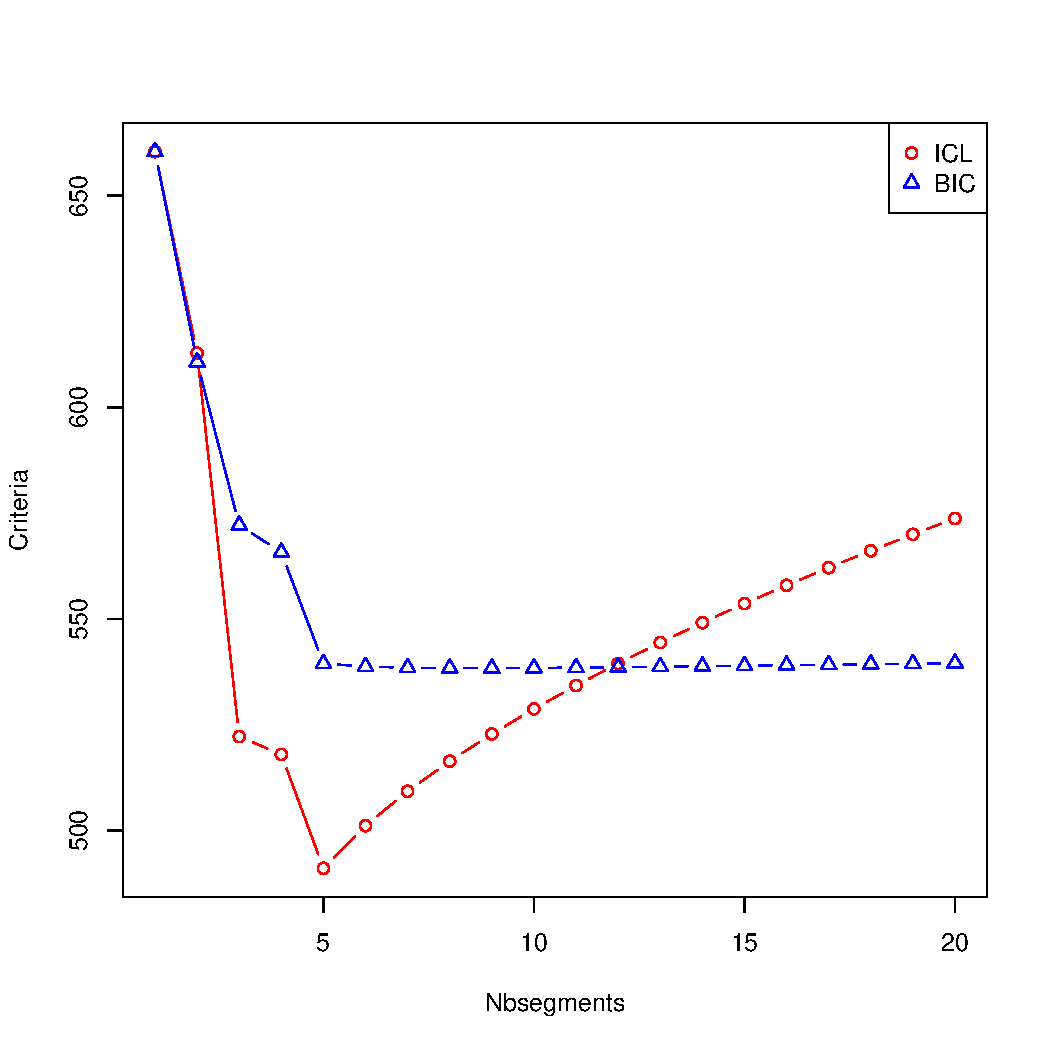
\includegraphics[width=6cm]{icl-bic.pdf}}
\caption{BIC and ICL criteria as a function of the number of segments} \label{fig:01}
\end{figure}






\subsection{Change-point location distribution}

Once the number of segments is chosen, one might be interested in the distribution of the location of each change-points. Two functions are implemented to address this question. \texttt{EBSDistrib} returns the distribution of the $k^{th}$ changepoint of a segmentation in $K$ segments. \texttt{EBSPlotProba} plots the distribution of all $K\!-\!1$ change-points of a segmentation in $K$ segments. The user has the option to plot those distributions on top of the data. 
\begin{verbatim}
> EBSPlotProba(out, Kicl, data=TRUE,
  file="my-segmentation.pdf")
\end{verbatim}

Figure \ref{fig:02} shows the output. 

\begin{figure}[!h]%figure1
\centerline{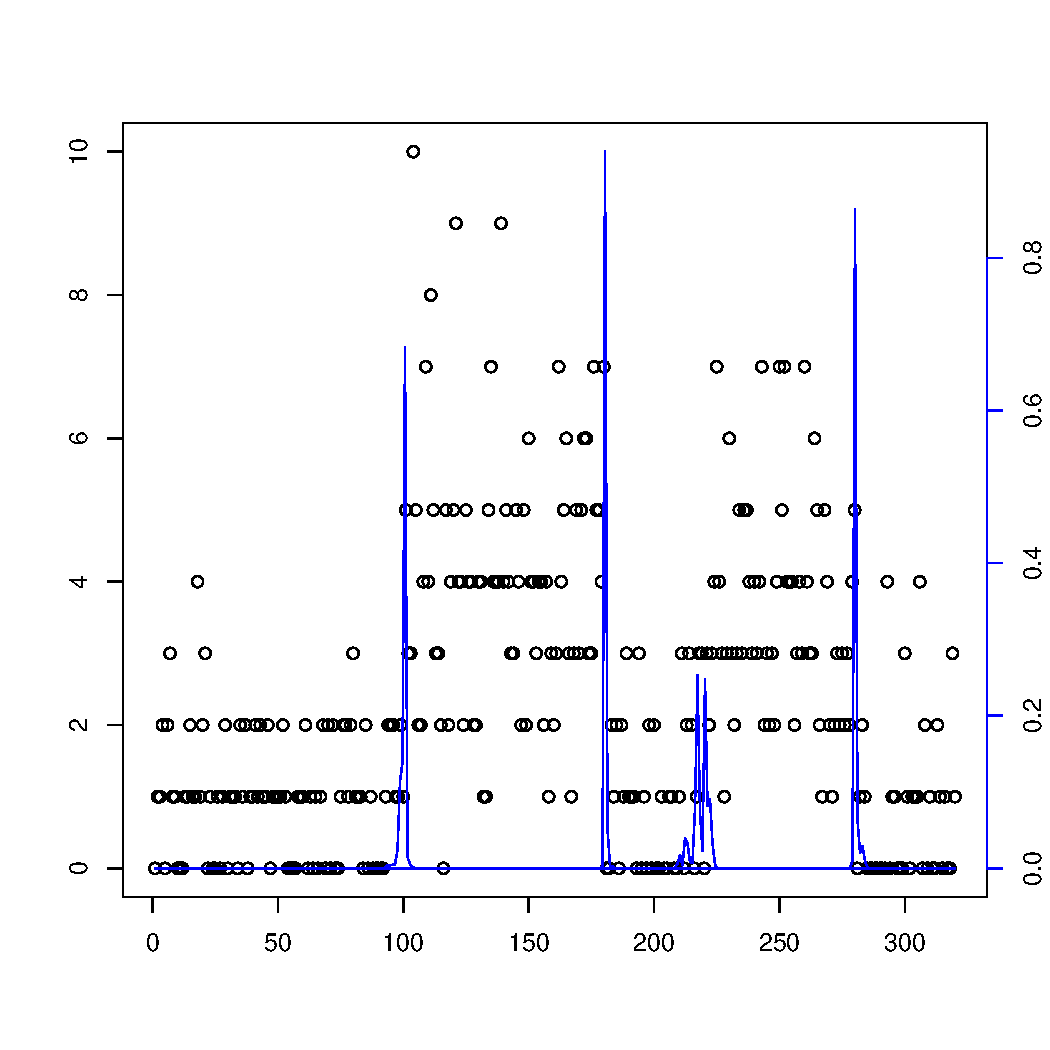
\includegraphics[width=6cm]{my-segmentation.pdf}}
\caption{file \textit{my-segmentation.pdf}, output of function \texttt{EBSPlotProba}}\label{fig:02}
\end{figure}

\end{methods}



\section{Implementation}

The preprocessing of the input data is handled by the R language,
giving the user easier access to a large amount of data. The model fitting, computation of probabilities 
and other time consuming operations are implemented in a versatile C++ code, and dynamically loaded into R.
Several methods are available for further analysis of the results. The package
offers various diagnostic tools and functions for visualization, for
example, plotting the breakpoint location distributions for a given number of segments.




\section{Conclusion}

This note introduces the EBS package for the analysis of NGS and CGH-array data. It allows a complete analysis of the segmentation space for biological profiles in an exact Bayesian framework. 
It provides an efficient criterion for the selection of the number of segments and allows further analysis of variables such as the entropy or the location of a change-point. 
Future improvements of the package include the analysis of other quantities of interest such as the posterior mean of the signal.



\section*{Acknowledgement}
We whish to thank Gregory Nuel and Michel Koskas for their help dealing with numerical issues.


%\bibliographystyle{natbib}
%\bibliographystyle{achemnat}
%\bibliographystyle{plainnat}
%\bibliographystyle{abbrv}
%\bibliographystyle{bioinformatics}
%
%\bibliographystyle{plain}
%
%\bibliography{Document}


\begin{thebibliography}{}

\bibitem[Bellman, 1961]{bellman_approximation_1961} Richard Bellman (1961) On the approximation of curves by line segments using dynamic programming,  {\it Commun. {ACM}}, {\bf 4}, 284.

\bibitem[Biernacki {\it et~al}., 2000]{biernacki_assessingmixture_2000} Biernacki, C., Celeux, G. and Govaert, G. (2000) Assessing a mixture model for clustering with the integrated completed likelihood, {\it{IEEE} Transactions on Pattern Analysis and Machine Intelligence}, {\bf 22} 719-725.

\bibitem[Breiman, 1984]{breiman_cart} Breiman, Friedman, Olshen and Stone (1984) Classification and Regression Trees, {\it Wadsworth and Brooks}.

\bibitem[Luong {\it et~al}, 2012]{Luong_HMM_2012} Luong, T.~M., Rozenholc, Y. and Nuel, G. (2012) Fast estimation of posterior probabilities in change-point models through a constrained hidden Markov model {http://adsabs.harvard.edu/abs/2012arXiv1203.4394L}.

\bibitem[Rigaill {\it et~al}., 2010]{rigaill_exact_2011} Rigaill, G., Lebarbier, E., Robin, S. (2011) Exact posterior distributions over the segmentation space and model selection for multiple change-point detection problems, {\it Statistics and Computing}, {\bf 22-4}, 917-929.

\end{thebibliography}
\end{document}
